\subsection{Scrumban: Implementación.}

La gestión eficiente del proceso de desarrollo constituye un factor determinante en el éxito de cualquier proyecto de software. Para este launcher, se adoptó el framework \textit{Scrumban}, una metodología híbrida que combina la estructura organizacional de Scrum con la flexibilidad visual de Kanban. Esta elección se fundamenta en la necesidad de mantener un desarrollo ágil y adaptativo, característico de Scrum, mientras se aprovecha la organización y visualización coherente de actividades que proporciona el tablero Kanban.

Scrumban resulta particularmente adecuado para proyectos individuales, donde la flexibilidad para ajustar prioridades y la capacidad de visualizar el flujo de trabajo son más importantes que las ceremonias tradicionales de Scrum.

\subsubsection{Sprints.}

El proceso de desarrollo se estableció en sprints de \textbf{dos (2) semanas} de duración, considerándose un ritmo sostenible que permitió la planificación detallada sin comprometer la flexibilidad del proceso. El cronograma de desarrollo se dividió en dos períodos académicos: la fase inicial comprendió desde el 16 de agosto hasta el 19 de diciembre de 2024, seguida de una pausa académica y la posterior reanudación el 21 de febrero de 2025, concluyendo el 29 de mayo de 2025. En total se ejecutaron \textbf{dieciseis (16) sprints} que abarcaron desde la conceptualización inicial hasta la implementación completa del launcher.

Los primeros sprints se dedicaron al modelado conceptual de la aplicación y la definición de requerimientos funcionales y no funcionales. Posteriormente, se desarrollaron los mockups y prototipos de interfaz con el objetivo de tener una base visual y de experiencia de usuario sólida para la siguiente etapa. Finalmente, los sprints restantes se enfocaron en la implementación del launcher utilizando Android Studio y las tecnologías previamente seleccionadas.

\subsubsection{Gestión de actividades: GitHub Projects.}

GitHub Projects fue seleccionada como plataforma de gestión de actividades debido a que ofrece una integración y comunicación directa con el repositorio de la aplicación alojado en GitHub y es extremadamente sencilla de utilizar y configurar para diferentes metodologías o tipos de proyectos. La configuración implementada en GitHub Projects incluyó la selección de la plantilla Kanban para reflejar el flujo de trabajo deseado. Se establecieron columnas que representan los estados del trabajo: \textbf{Backlog, En progreso, En revisión, Completado y Listo}, como se muestra en la Figura \ref{fig:github_projects_tablero_kanban}.

\begin{figure}[ht]
  \caption{Tablero Kanban de GitHub Projects.}
  \label{fig:github_projects_tablero_kanban}
  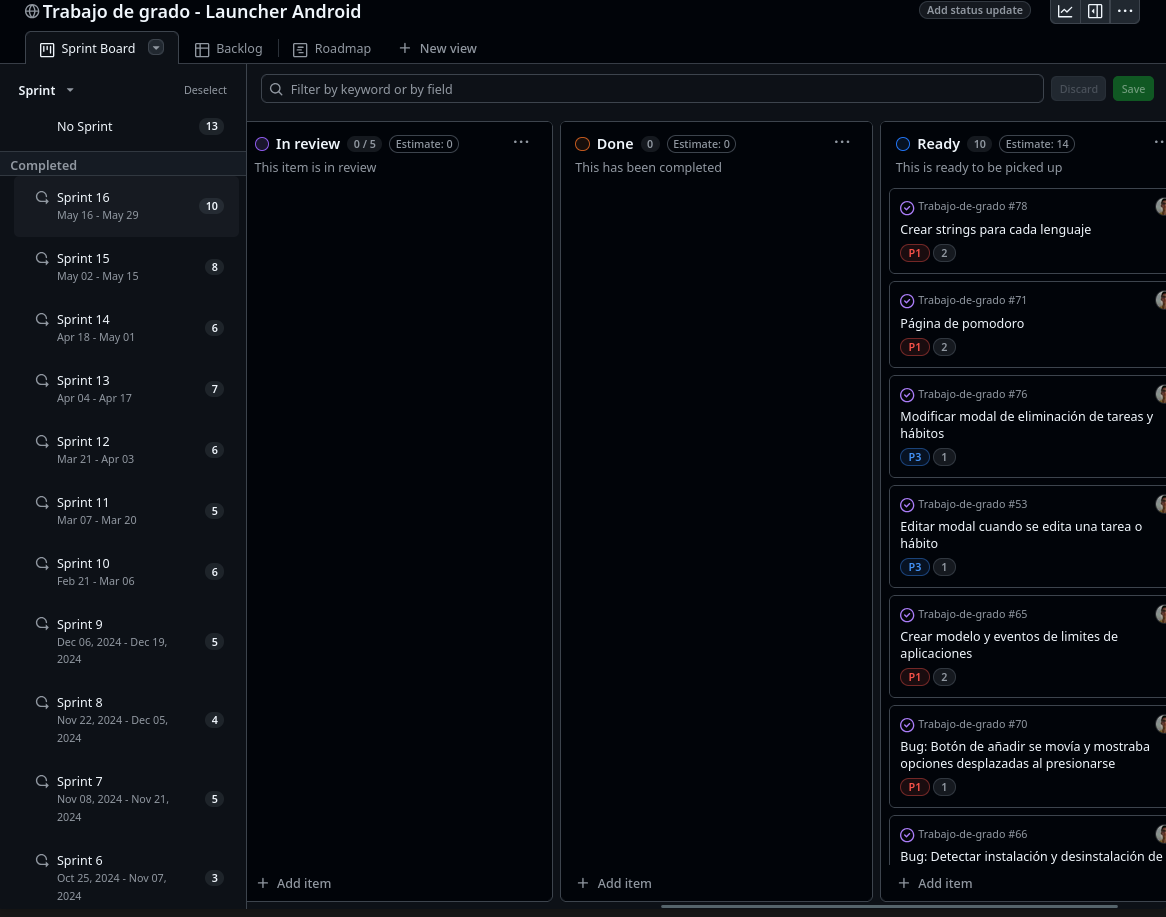
\includegraphics[width=\textwidth]{Figuras/github_projects_tablero_kanban.png}
  \centering
\end{figure}

Las historias de usuario se consignaron en el backlog de GitHub Projects al inicio del proyecto y cada vez que se requería corregir un error o agregar una funcionalidad que no estaba contemplada al inicio del proyecto. Cada historia siguió la estructura estándar de metodologías ágiles: 

\begin{quote}
\centering
\texttt{Como [tipo de usuario],}
\newline
\texttt{quiero [acción]}
\newline
\texttt{para [beneficio].}
\end{quote}

Para historias de mayor complejidad o con aspectos técnicos específicos, se incluyeron criterios de aceptación detallados que establecen las condiciones que deben cumplirse para considerar la funcionalidad como completamente implementada. En la Figura \ref{fig:historia_de_usuario_1}, Figura \ref{fig:historia_de_usuario_2} y Figura \ref{fig:historia_de_usuario_3} se muestran algunos ejemplos de historias de usuario. Para ver la lista completa de historias de usuario, consultar el proyecto en \url{https://github.com/users/Juansebas064/projects/3/views/6}.

\begin{figure}[ht]
  \caption{Ejemplo 1: Historia de usuario.}
  \label{fig:historia_de_usuario_1}
  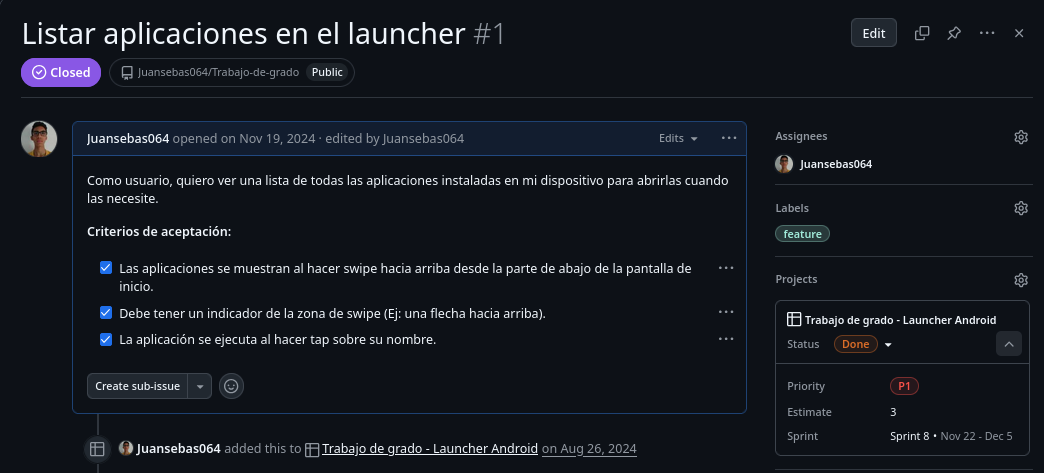
\includegraphics[width=\textwidth]{Figuras/historia_de_usuario_1.png}
  \centering
\end{figure}

\begin{figure}[ht]
  \caption{Ejemplo 2: Historia de usuario.}
  \label{fig:historia_de_usuario_2}
  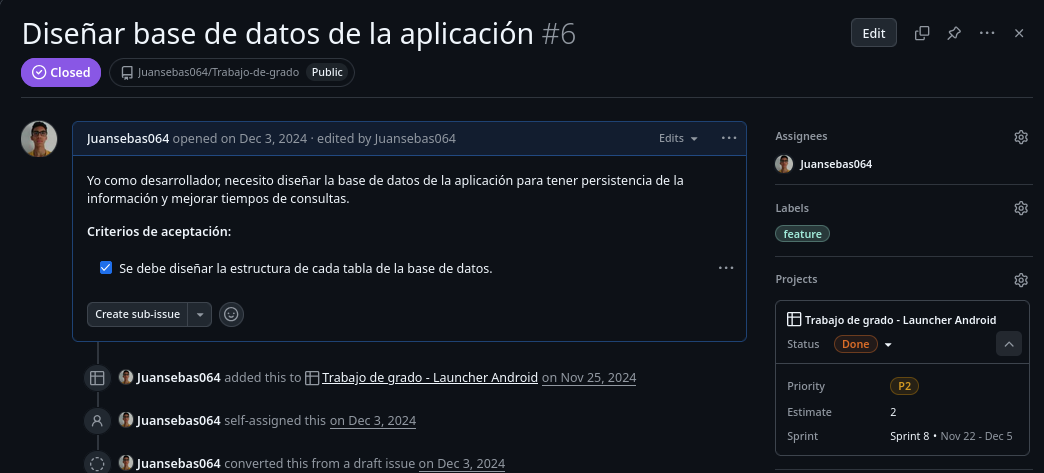
\includegraphics[width=\textwidth]{Figuras/historia_de_usuario_2.png}
  \centering
\end{figure}

\begin{figure}[ht]
  \caption{Ejemplo 3: Historia de usuario.}
  \label{fig:historia_de_usuario_3}
  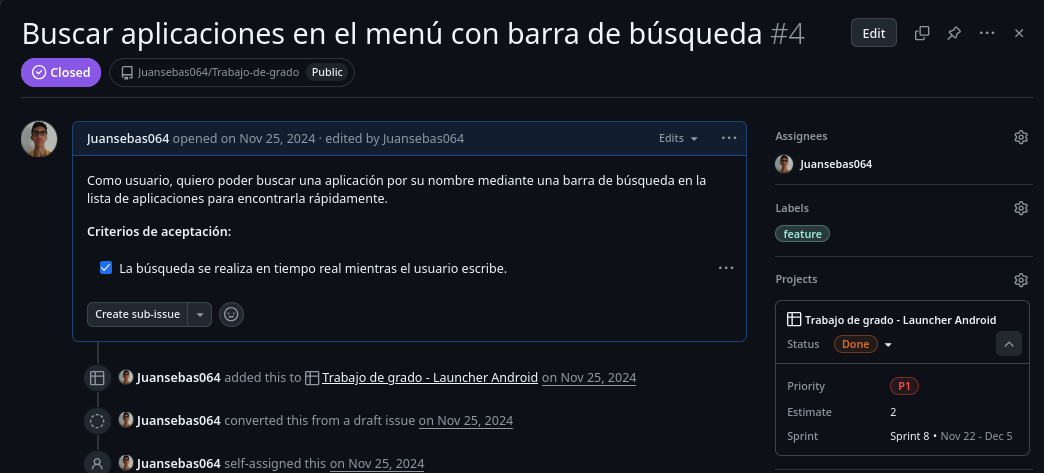
\includegraphics[width=\textwidth]{Figuras/historia_de_usuario_3.png}
  \centering
\end{figure}

\subsubsection{GitHub Flow.}

\textit{GitHub Flow} es una metodología de control de versiones y colaboración en desarrollo de software que se caracteriza por su simplicidad y enfoque en la entrega continua. Desarrollada por GitHub como una alternativa más ágil y menos compleja que \textit{Git Flow}, esta metodología se fundamenta en un flujo de trabajo lineal que prioriza la rapidez de integración y el despliegue frecuente de cambios. La filosofía central de GitHub Flow se basa en mantener la rama principal (main) siempre en un estado desplegable, lo que significa que cualquier código que se integre a esta rama debe estar completamente funcional y listo para producción.

Se buscó que la gestión del proyecto fuera simple pero con una estructura bien definida, este flujo de trabajo se adaptó perfectamente a las necesidades de estandarizar la gestión de ramas de \textit{Git} y de integrar de manera continua los cambios con la rama principal. El proceso de GitHub Flow se estructura en seis pasos: \textbf{Primero}, se crea una nueva rama a partir de la rama principal para cada nueva funcionalidad, corrección de errores o mejora que se desee implementar. Esta rama debe tener un nombre descriptivo (ejemplo: \texttt{apps-limit}) que refleje claramente el propósito del trabajo a realizar.

\textbf{Segundo}, se realizan los commits necesarios en esta rama de trabajo, manteniendo un historial claro y conciso de los cambios implementados.

\textbf{Tercero}, se abre un \textit{Pull Request (PR)} hacia la rama principal, iniciando el proceso de revisión de código. El PR actúa como mecanismo de documentación y discusión sobre los cambios propuestos y protege a la rama principal de ser directamente modificada.

\textbf{Cuarto}, se lleva a cabo la revisión del código en el PR, donde otros miembros del equipo (en el caso de haber varios) evalúan la calidad, funcionalidad y adherencia a los estándares establecidos.

\textbf{Quinto}, una vez que el PR ha sido aprobado y todas las verificaciones automáticas han pasado exitosamente, se procede a la integración del código en la rama principal mediante un \textit{merge}.

\textbf{Sexto}, inmediatamente después de la integración, se procede al despliegue de los cambios en el ambiente de producción, aprovechando que la rama principal se mantiene siempre en estado desplegable (en este caso, la instalación en el dispositivo Android).

En la Figura \ref{fig:ramas_de_github} podemos ver algunas de las ramas que se utilizaron a lo largo del desarrollo del launcher.
\begin{figure}[ht]
  \caption{Gestión de ramas con GitHub Flow.}
  \label{fig:ramas_de_github}
  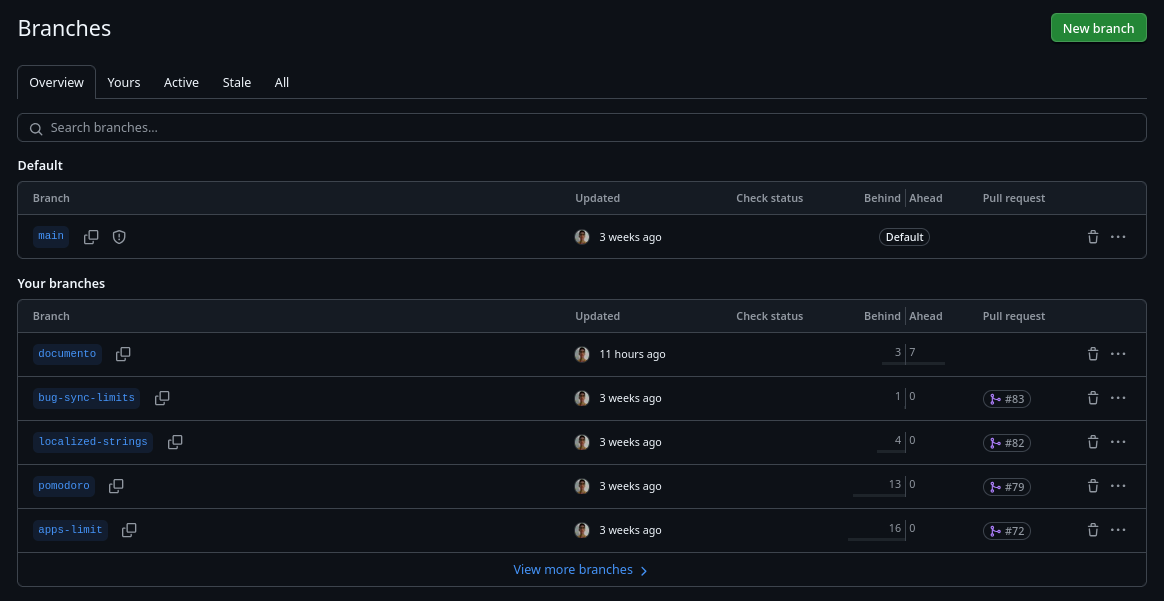
\includegraphics[width=\textwidth]{Figuras/ramas_de_github.png}
  \centering
\end{figure}